\ifx\pdfminorversion\undefined\else\pdfminorversion=4\fi
\documentclass[aspectratio=43,t]{beamer}
%\documentclass[aspectratio=43,t,handout]{beamer}

% English version FAU Logo
%\usepackage[english]{babel}
% German version FAU Logo
\usepackage[ngerman]{babel}

\usepackage[utf8]{inputenc}
\usepackage[T1]{fontenc}
\usepackage{amsmath,amssymb}
\usepackage{graphicx}
\usepackage{minted}
\usepackage{subcaption}
\usepackage[export]{adjustbox}
\usepackage[backend=biber,sorting=none,doi=true,style=ieee]{biblatex}

\setminted{fontsize=\scriptsize}
% Options:
%  - inst:      Institute
%                 med:      MedFak FAU theme
%                 nat:      NatFak FAU theme
%                 phil:     PhilFak FAU theme
%                 rw:       RWFak FAU theme
%                 rw-jura:  RWFak FB Jura FAU theme
%                 rw-wiso:  RWFak FB WISO FAU theme
%                 tf:       TechFak FAU theme
%                 tf-hscd:  TechFak Co-Design FAU theme
%  - image:     Cover image on title page
%  - plain:     Plain title page
%  - longtitle: Title page layout for long title
\usetheme[%
  inst=tf-hscd,%
  longtitle%
]{fau}

% Enable semi-transparent animation preview
\setbeamercovered{transparent}

\defbibheading{bibliography}{}
\addbibresource[label=primary]{references.bib}
\nocite{*}


% Title, authors, and date
\title[Backtracking]{Backtracking}
\subtitle{Ausgewählte Kapitel aus "The Art of Computer Programming"}
\author[Bastian Kauschke]{Bastian Kauschke}
% English version
%\institute[Hardware/Software Co-Design]{Hardware/Software Co-Design, Friedrich-Alexander University Erlangen-Nürnberg}
% German version
\institute[Hardware-Software-Co-Design]{Hardware-Software-Co-Design, Friedrich-Alexander-Universität Erlangen-Nürnberg}
\date{\today}
% Set additional logo (overwrites FAU seal)
%\logo{
\includegraphics[width=.15\textwidth]{themefau/art/tf/hscd/codesign.pdf}}


\begin{document}
  % Title
  \maketitle

  { % Outline
    \setbeamertemplate{footline}{}
    \begin{frame}[noframenumbering]{Outline}
      \tableofcontents
    \end{frame}
  }

  % Body
  \section{Einführung}
  \begin{frame}{Anwendungsbereich}
    Sequenzen $x_{1}, x_{2}, x_{3} \dots x_{n}$ für welche die Bedingung $P_{n}(x_{1}, x_{2}, x_{3} \dots x_{n})$ gilt.\\
    \ \\ 
    $P$ hat dabei folgende Eigenschaften: \pause
    \begin{itemize}
      \item $P_{l}(x_{1}, x_{2}, x_{3} \dots x_{l})$ gilt nur, wenn $P_{l-1}(x_{1}, x_{2}, x_{3} \dots x_{l-1})$ gilt \pause
      \item wenn $P_{l}(x_{1}, x_{2}, x_{3} \dots x_{l})$ gilt, ist $P_{l+1}(x_{1}, x_{2}, x_{3} \dots x_{l+1})$ einfach zu testen \pause
      \item $P_{0}()$ gilt immer
    \end{itemize}
  \end{frame}

  \begin{frame}[fragile]{Algorithmus}
    \begin{minted}{rust}
/// A required set of methods needed for the generic backtracking algorithms.
pub trait Sequence {
    type Step;
    type Steps: IntoIterator<Item = Self::Step>;

    /// Checks if this sequence satisfy its condition.
    ///
    /// This function can assume that the  parent of `self` satisfied this condition.
    fn satisfies_condition(&self) -> bool;

    /// generates all possible next steps at this current state.
    fn next_steps(&self) -> Self::Steps;

    /// applies a `step` to `self`, returning the resulting sequence.
    ///
    /// this function will only be called if `self.satisfies_condition() == true`.
    fn apply_step(&self, step: Self::Step) -> Self;
}

      \end{minted}
    \end{frame}
    \begin{frame}[fragile]{Algorithmus}
      \begin{minted}{rust}
pub fn b<T: Sequence>(initial: T, n: usize) -> Vec<T> {
    let mut results = Vec::new();
    let mut states = Vec::new();
    let steps = initial.next_steps().into_iter();
    states.push((initial, steps));

    while let Some((state, steps)) = states.last_mut() {
        if let Some(step) = steps.next() {
            let next_state = state.apply_step(step);
            if next_state.satisfies_condition() {
                if states.len() < n {
                    let next_steps = next_state.next_steps().into_iter();
                    states.push((next_state, next_steps));
                } else {
                    results.push(next_state);
                }
            }
        } else {
            states.pop();
        }
    }
    results
}
    \end{minted}
  \end{frame}
  \section{n Queens}
    \begin{frame}{Damenproblem}
      Wie kann man $n$ Damen auf einem $n * n$ Schachbrett aufstellen, ohne dass sich zwei Damen schlagen können, 
      also keine 2 Damen in der selben Zeile, Reihe oder Diagonalen stehen.
      \begin{figure}[h!]
        \centering
        \begin{subfigure}{0.4\linewidth}
          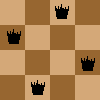
\includegraphics[width=\linewidth]{../img/queensRight.png}
          \caption{Richtig}
        \end{subfigure}
        \begin{subfigure}{0.4\linewidth}
          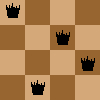
\includegraphics[width=\linewidth]{../img/queensWrong.png}
          \caption{Falsch}
        \end{subfigure}
        \label{n4}
      \end{figure}
    \end{frame}
    \begin{frame}{impl Sequence}
      \begin{center}
        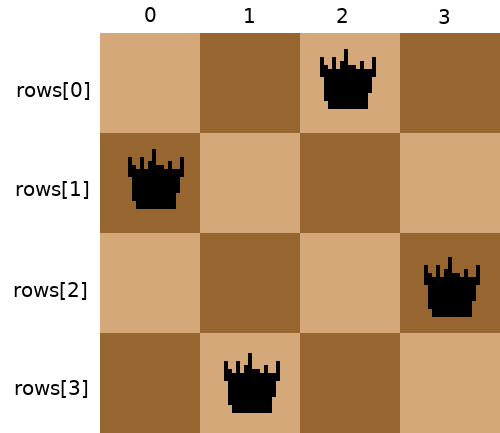
\includegraphics[width=\textwidth,height=0.8\textheight,keepaspectratio]{../img/q4.png}
      \end{center}
    \end{frame}
    \begin{frame}[fragile]{impl Sequence}
      \begin{minted}[fontsize=\normalsize]{rust}
pub struct Queens {
    n: usize,
    rows: Vec<usize>,
}

impl Queens {
    pub fn new(n: usize) -> Self {
        Self {
            n,
            rows: Vec::new(),
        }
    }
}
      \end{minted}
    \end{frame}
    \begin{frame}[fragile]{impl Sequence}
\begin{minted}[fontsize=\small]{rust}
fn satisfies_condition(&self) -> bool {
    if self.rows.is_empty() {
        return true;
    }

    let k = self.rows.len() - 1;

    for j in 0..k {
        let k_col = self.rows[k] as isize;
        let j_col = self.rows[j] as isize;

        if k_col == j_col || (j_col - k_col).abs() as usize == k - j {
            return false;
        }
    }
    true
}
\end{minted}
    \end{frame}
    \begin{frame}[fragile]{impl Sequence}
\begin{minted}[fontsize=\normalsize]{rust}
fn next_steps(&self) -> Self::Steps {
    0..self.n
}

fn apply_step(&self, step: Self::Step) -> Self {
    let mut rows = self.rows.clone();
    rows.push(step);
    Self { n: self.n, rows }
}
\end{minted}
    \end{frame}

    \begin{frame}[fragile]
    \begin{minted}[fontsize=\normalsize]{rust}
let results = b(Queens::new(4), 4);

pub fn b<T: Sequence>(initial: T, n: usize) -> Vec<T> {
    let mut results = Vec::new();
    let mut states = Vec::new();

    let steps = initial.next_steps().into_iter();
    states.push((initial, steps));
    // <- we are here
    // ...
}
    \end{minted}
    \ \\
    $results = [\ ]$ \\
    \ \\
    $states = [(\raisebox{-2ex}{
\includegraphics[height=\baselineskip * 2]{../img/empty.png}}, [
    
\includegraphics[height=\baselineskip / 2]{../img/step0.png},
    
\includegraphics[height=\baselineskip / 2]{../img/step1.png},
    
\includegraphics[height=\baselineskip / 2]{../img/step2.png},
    
\includegraphics[height=\baselineskip / 2]{../img/step3.png}])]$
\end{frame}
\begin{frame}[fragile]
    \begin{minted}{rust}
// ...
while let Some((state, steps)) = states.last_mut() {
    if let Some(step) = steps.next() {
        // <- we are here
        let next_state = state.apply_step(step);
        if next_state.satisfies_condition() {
            if states.len() < n {
                let next_steps = next_state.next_steps().into_iter();
                states.push((next_state, next_steps));
            } else {
                results.push(next_state);
            }
        }
    } else {
        states.pop();
    }
}
// ...
    \end{minted}
    $states = [(\raisebox{-2ex}{
\includegraphics[height=\baselineskip * 2]{../img/empty.png}}, [
    
\includegraphics[height=\baselineskip / 2]{../img/step1.png},
    
\includegraphics[height=\baselineskip / 2]{../img/step2.png},
    
\includegraphics[height=\baselineskip / 2]{../img/step3.png}])]$
    \ \\
    $step = 
\includegraphics[height=\baselineskip / 2]{../img/step0.png}$
\end{frame}
\begin{frame}[fragile]
    \begin{minted}{rust}
// ...
while let Some((state, steps)) = states.last_mut() {
    if let Some(step) = steps.next() {
        let next_state = state.apply_step(step);
        // <- we are here
        if next_state.satisfies_condition() {
            if states.len() < n {
                let next_steps = next_state.next_steps().into_iter();
                states.push((next_state, next_steps));
            } else {
                results.push(next_state);
            }
        }
    } else {
        states.pop();
    }
}
// ...
    \end{minted}
    $states = [(\raisebox{-2ex}{
\includegraphics[height=\baselineskip * 2]{../img/empty.png}}, [
    
\includegraphics[height=\baselineskip / 2]{../img/step1.png},
    
\includegraphics[height=\baselineskip / 2]{../img/step2.png},
    
\includegraphics[height=\baselineskip / 2]{../img/step3.png}])]$
    \ \\
    $next\_state = \raisebox{-2ex}{
\includegraphics[height=\baselineskip * 2]{../img/state0.png}}$
\end{frame}
\begin{frame}[fragile]
    \begin{minted}{rust}
// ...
while let Some((state, steps)) = states.last_mut() {
    if let Some(step) = steps.next() {
        let next_state = state.apply_step(step);
        // our previous position
        if next_state.satisfies_condition() {
            if states.len() < n {
                let next_steps = next_state.next_steps().into_iter();
                states.push((next_state, next_steps));
                // <- we are here
            } else {
                results.push(next_state);
            }
        }
    } else {
        states.pop();
    }
}
// ...
    \end{minted}
    $states = [(\raisebox{-2ex}{
\includegraphics[height=\baselineskip * 2]{../img/empty.png}}, [
    
\includegraphics[height=\baselineskip / 2]{../img/step1.png},
    
\includegraphics[height=\baselineskip / 2]{../img/step2.png},
    
\includegraphics[height=\baselineskip / 2]{../img/step3.png}]),
    (\raisebox{-2ex}{
\includegraphics[height=\baselineskip * 2]{../img/state0.png}}, [
    
\includegraphics[height=\baselineskip / 2]{../img/step0.png},
    
\includegraphics[height=\baselineskip / 2]{../img/step1.png},
    
\includegraphics[height=\baselineskip / 2]{../img/step2.png},
    
\includegraphics[height=\baselineskip / 2]{../img/step3.png}])]$
\end{frame}
\begin{frame}[fragile]
    \begin{minted}{rust}
// ...
while let Some((state, steps)) = states.last_mut() {
    if let Some(step) = steps.next() {
        let next_state = state.apply_step(step);
        // <- we are here
        if next_state.satisfies_condition() {
            if states.len() < n {
                let next_steps = next_state.next_steps().into_iter();
                states.push((next_state, next_steps));
            } else {
                results.push(next_state);
            }
        }
    } else {
        states.pop();
    }
}
// ...
    \end{minted}
    $states = [(\raisebox{-2ex}{
\includegraphics[height=\baselineskip * 2]{../img/empty.png}}, [
    
\includegraphics[height=\baselineskip / 2]{../img/step1.png},
    
\includegraphics[height=\baselineskip / 2]{../img/step2.png},
    
\includegraphics[height=\baselineskip / 2]{../img/step3.png}]),
    (\raisebox{-2ex}{
\includegraphics[height=\baselineskip * 2]{../img/state0.png}}, [
    
\includegraphics[height=\baselineskip / 2]{../img/step1.png},
    
\includegraphics[height=\baselineskip / 2]{../img/step2.png},
    
\includegraphics[height=\baselineskip / 2]{../img/step3.png}])]$ \ \\
    $next\_state = \raisebox{-2ex}{
\includegraphics[height=\baselineskip * 2]{../img/state00.png}}$
\end{frame}
\begin{frame}[fragile]
    \begin{minted}{rust}
// ...
while let Some((state, steps)) = states.last_mut() {
    if let Some(step) = steps.next() {
        let next_state = state.apply_step(step);
        // <- we are here
        if next_state.satisfies_condition() {
            if states.len() < n {
                let next_steps = next_state.next_steps().into_iter();
                states.push((next_state, next_steps));
            } else {
                results.push(next_state);
            }
        }
    } else {
        states.pop();
    }
}
// ...
    \end{minted}
    $states = [(\raisebox{-2ex}{
\includegraphics[height=\baselineskip * 2]{../img/empty.png}}, [
    
\includegraphics[height=\baselineskip / 2]{../img/step1.png},
    
\includegraphics[height=\baselineskip / 2]{../img/step2.png},
    
\includegraphics[height=\baselineskip / 2]{../img/step3.png}]),
    (\raisebox{-2ex}{
\includegraphics[height=\baselineskip * 2]{../img/state0.png}}, [
    
\includegraphics[height=\baselineskip / 2]{../img/step2.png},
    
\includegraphics[height=\baselineskip / 2]{../img/step3.png}])]$ \ \\
    $next\_state = \raisebox{-2ex}{
\includegraphics[height=\baselineskip * 2]{../img/state01.png}}$
\end{frame}
\begin{frame}[fragile]
    \begin{minted}{rust}
// ...
while let Some((state, steps)) = states.last_mut() {
    if let Some(step) = steps.next() {
        let next_state = state.apply_step(step);
        // <- we are here
        if next_state.satisfies_condition() {
            if states.len() < n {
                let next_steps = next_state.next_steps().into_iter();
                states.push((next_state, next_steps));
            } else {
                results.push(next_state);
            }
        }
    } else {
        states.pop();
    }
}
// ...
    \end{minted}
    $states = [(\raisebox{-2ex}{
\includegraphics[height=\baselineskip * 2]{../img/empty.png}}, [
    
\includegraphics[height=\baselineskip / 2]{../img/step1.png},
    
\includegraphics[height=\baselineskip / 2]{../img/step2.png},
    
\includegraphics[height=\baselineskip / 2]{../img/step3.png}]),
    (\raisebox{-2ex}{
\includegraphics[height=\baselineskip * 2]{../img/state0.png}}, [
    \includegraphics[height=\baselineskip / 2]{../img/step3.png}])]$ \ \\
    $next\_state = \raisebox{-2ex}{\includegraphics[height=\baselineskip * 2]{../img/state02.png}}$
\end{frame}
\begin{frame}[fragile]
    \begin{minted}{rust}
while let Some((state, steps)) = states.last_mut() {
    if let Some(step) = steps.next() {
        let next_state = state.apply_step(step);
        if next_state.satisfies_condition() {
            if states.len() < n {
                let next_steps = next_state.next_steps().into_iter();
                states.push((next_state, next_steps));
                // <- we are here
            } else {
                results.push(next_state);
            }
        }
    } else {
        states.pop();
    }
}
    \end{minted}
    $states = [(\raisebox{-2ex}{\includegraphics[height=\baselineskip * 2]{../img/empty.png}}, [
    \includegraphics[height=\baselineskip / 2]{../img/step1.png},
    \includegraphics[height=\baselineskip / 2]{../img/step2.png},
    \includegraphics[height=\baselineskip / 2]{../img/step3.png}]
    ),
    (\raisebox{-2ex}{\includegraphics[height=\baselineskip * 2]{../img/state0.png}}, [
    \includegraphics[height=\baselineskip / 2]{../img/step3.png}]
    ), \\
    (\raisebox{-2ex}{\includegraphics[height=\baselineskip * 2]{../img/state02.png}}, [
    \includegraphics[height=\baselineskip / 2]{../img/step0.png},
    \includegraphics[height=\baselineskip / 2]{../img/step1.png},
    \includegraphics[height=\baselineskip / 2]{../img/step2.png},
    \includegraphics[height=\baselineskip / 2]{../img/step3.png}]
    )]$ \ \\
\end{frame}
\begin{frame}[fragile]
    \begin{minted}{rust}
while let Some((state, steps)) = states.last_mut() {
    // <- we are here after discarding all 4 steps
    if let Some(step) = steps.next() {
        let next_state = state.apply_step(step);
        if next_state.satisfies_condition() {
            if states.len() < n {
                let next_steps = next_state.next_steps().into_iter();
                states.push((next_state, next_steps));
            } else {
                results.push(next_state);
            }
        }
    } else {
        states.pop();
    }
}
    \end{minted}
    $states = [(\raisebox{-2ex}{\includegraphics[height=\baselineskip * 2]{../img/empty.png}}, [
    \includegraphics[height=\baselineskip / 2]{../img/step1.png},
    \includegraphics[height=\baselineskip / 2]{../img/step2.png},
    \includegraphics[height=\baselineskip / 2]{../img/step3.png}]
    ),
    (\raisebox{-2ex}{\includegraphics[height=\baselineskip * 2]{../img/state0.png}}, [
    \includegraphics[height=\baselineskip / 2]{../img/step3.png}]
    ),
    (\raisebox{-2ex}{\includegraphics[height=\baselineskip * 2]{../img/state02.png}}, [\ ])]$ \ \\
\end{frame}
\begin{frame}[fragile]
    \begin{minted}{rust}
while let Some((state, steps)) = states.last_mut() {
    if let Some(step) = steps.next() {
        let next_state = state.apply_step(step);  
        if next_state.satisfies_condition() {
            if states.len() < n {
                let next_steps = next_state.next_steps().into_iter();
                states.push((next_state, next_steps));
            } else {
                results.push(next_state);
            }
        }
    } else {
        states.pop();
        // <- we are here
    }
}
    \end{minted}
    $states = [(\raisebox{-2ex}{\includegraphics[height=\baselineskip * 2]{../img/empty.png}}, [
    \includegraphics[height=\baselineskip / 2]{../img/step1.png},
    \includegraphics[height=\baselineskip / 2]{../img/step2.png},
    \includegraphics[height=\baselineskip / 2]{../img/step3.png}]
    ),
    (\raisebox{-2ex}{\includegraphics[height=\baselineskip * 2]{../img/state0.png}}, [
    \includegraphics[height=\baselineskip / 2]{../img/step3.png}]
    )]$ \ \\
\end{frame}
\begin{frame}[fragile]
    \begin{minted}{rust}
while let Some((state, steps)) = states.last_mut() {
    if let Some(step) = steps.next() {
        let next_state = state.apply_step(step);
        // <- we are here
        if next_state.satisfies_condition() {
            if states.len() < n {
                let next_steps = next_state.next_steps().into_iter();
                states.push((next_state, next_steps));
            } else {
                results.push(next_state);
            }
        }
    } else {
        states.pop();
    }
}
    \end{minted}
    $states = [(\raisebox{-2ex}{\includegraphics[height=\baselineskip * 2]{../img/empty.png}}, [
    \includegraphics[height=\baselineskip / 2]{../img/step1.png},
    \includegraphics[height=\baselineskip / 2]{../img/step2.png},
    \includegraphics[height=\baselineskip / 2]{../img/step3.png}]
    ),
    (\raisebox{-2ex}{\includegraphics[height=\baselineskip * 2]{../img/state0.png}}, [\ ])]$ \ \\
    $next\_state = \raisebox{-2ex}{\includegraphics[height=\baselineskip * 2]{../img/state03.png}}$
\end{frame}
\begin{frame}[fragile]
    \begin{minted}{rust}
while let Some((state, steps)) = states.last_mut() {
    if let Some(step) = steps.next() {
        let next_state = state.apply_step(step);
        // <- we are here
        if next_state.satisfies_condition() {
            if states.len() < n {
                let next_steps = next_state.next_steps().into_iter();
                states.push((next_state, next_steps));
            } else {
                results.push(next_state);
            }
        }
    } else {
        states.pop();
    }
}
    \end{minted}
    $states = [(\raisebox{-2ex}{\includegraphics[height=\baselineskip * 2]{../img/empty.png}}, [
    \includegraphics[height=\baselineskip / 2]{../img/step1.png},
    \includegraphics[height=\baselineskip / 2]{../img/step2.png},
    \includegraphics[height=\baselineskip / 2]{../img/step3.png}]
    ),
    (\raisebox{-2ex}{\includegraphics[height=\baselineskip * 2]{../img/state0.png}}, [\ ]),
    (\raisebox{-2ex}{\includegraphics[height=\baselineskip * 2]{../img/state03.png}}, [
    \includegraphics[height=\baselineskip / 2]{../img/step2.png},
    \includegraphics[height=\baselineskip / 2]{../img/step3.png}])]$ \ \\
    $next\_state = \raisebox{-2ex}{\includegraphics[height=\baselineskip * 2]{../img/state031.png}}$
\end{frame}
\begin{frame}[fragile]
    \begin{minted}{rust}
while let Some((state, steps)) = states.last_mut() {
    if let Some(step) = steps.next() {
        let next_state = state.apply_step(step);
        if next_state.satisfies_condition() {
            if states.len() < n {
                let next_steps = next_state.next_steps().into_iter();
                states.push((next_state, next_steps));
            } else {
                results.push(next_state);
            }
        }
    } else { 
        states.pop();
        // <- we are here
    }
}
    \end{minted}
    $states = [(\raisebox{-2ex}{\includegraphics[height=\baselineskip * 2]{../img/empty.png}}, [
    \includegraphics[height=\baselineskip / 2]{../img/step1.png},
    \includegraphics[height=\baselineskip / 2]{../img/step2.png},
    \includegraphics[height=\baselineskip / 2]{../img/step3.png}]
    ),
    (\raisebox{-2ex}{\includegraphics[height=\baselineskip * 2]{../img/state0.png}}, [\ ]),
    (\raisebox{-2ex}{\includegraphics[height=\baselineskip * 2]{../img/state03.png}}, [
    \includegraphics[height=\baselineskip / 2]{../img/step2.png},
    \includegraphics[height=\baselineskip / 2]{../img/step3.png}])]$ \ \\
\end{frame}
\begin{frame}[fragile]
    \begin{minted}{rust}
while let Some((state, steps)) = states.last_mut() {
    if let Some(step) = steps.next() {
        let next_state = state.apply_step(step);
        if next_state.satisfies_condition() {
            if states.len() < n {
                let next_steps = next_state.next_steps().into_iter();
                states.push((next_state, next_steps));
            } else {
                results.push(next_state);
            }
        }
    } else { 
        states.pop();
        // <- we are here
    }
}
    \end{minted}
    $states = [(\raisebox{-2ex}{\includegraphics[height=\baselineskip * 2]{../img/empty.png}}, [
    \includegraphics[height=\baselineskip / 2]{../img/step1.png},
    \includegraphics[height=\baselineskip / 2]{../img/step2.png},
    \includegraphics[height=\baselineskip / 2]{../img/step3.png}]
    ),
    (\raisebox{-2ex}{\includegraphics[height=\baselineskip * 2]{../img/state0.png}}, [\ ]),]$ \ \\
\end{frame}
\begin{frame}[fragile]
    \begin{minted}{rust}
while let Some((state, steps)) = states.last_mut() {
    if let Some(step) = steps.next() {
        let next_state = state.apply_step(step);
        if next_state.satisfies_condition() {
            if states.len() < n {
                let next_steps = next_state.next_steps().into_iter();
                states.push((next_state, next_steps));
                // <- we are here
            } else {
                results.push(next_state);
            }
        }
    } else { 
        states.pop();
    }
}
    \end{minted}
    $states = [(\raisebox{-2ex}{\includegraphics[height=\baselineskip * 2]{../img/empty.png}}, [
    \includegraphics[height=\baselineskip / 2]{../img/step2.png},
    \includegraphics[height=\baselineskip / 2]{../img/step3.png}]
    ),
    (\raisebox{-2ex}{\includegraphics[height=\baselineskip * 2]{../img/state1.png}}, [
    \includegraphics[height=\baselineskip / 2]{../img/step0.png},
    \includegraphics[height=\baselineskip / 2]{../img/step1.png},
    \includegraphics[height=\baselineskip / 2]{../img/step2.png},
    \includegraphics[height=\baselineskip / 2]{../img/step3.png}])]$ \ \\
\end{frame}
\begin{frame}[fragile]
    \begin{minted}{rust}
while let Some((state, steps)) = states.last_mut() {
    if let Some(step) = steps.next() {
        let next_state = state.apply_step(step);
        if next_state.satisfies_condition() {
            // <- we are here
            if states.len() < n {
                let next_steps = next_state.next_steps().into_iter();
                states.push((next_state, next_steps));
            } else {
                results.push(next_state);
            }
        }
    } else { 
        states.pop();
    }
}
    \end{minted}
    $states = [(\raisebox{-2ex}{\includegraphics[height=\baselineskip * 2]{../img/empty.png}}, [
    \includegraphics[height=\baselineskip / 2]{../img/step2.png},
    \includegraphics[height=\baselineskip / 2]{../img/step3.png}]
    ),
    (\raisebox{-2ex}{\includegraphics[height=\baselineskip * 2]{../img/state1.png}}, [\ ]),
    (\raisebox{-2ex}{\includegraphics[height=\baselineskip * 2]{../img/state13.png}}, [
    \includegraphics[height=\baselineskip / 2]{../img/step1.png},
    \includegraphics[height=\baselineskip / 2]{../img/step2.png},
    \includegraphics[height=\baselineskip / 2]{../img/step3.png}]
    ), \\
    (\raisebox{-2ex}{\includegraphics[height=\baselineskip * 2]{../img/state130.png}}, [
    \includegraphics[height=\baselineskip / 2]{../img/step3.png}]
    )]$ \ \\
    $next\_state = \raisebox{-2ex}{\includegraphics[height=\baselineskip * 2]{../img/state1302.png}}$
\end{frame}
\begin{frame}[fragile]
    \begin{minted}{rust}
while let Some((state, steps)) = states.last_mut() {
    if let Some(step) = steps.next() {
        let next_state = state.apply_step(step);
        if next_state.satisfies_condition() {
            if states.len() < n {
                let next_steps = next_state.next_steps().into_iter();
                states.push((next_state, next_steps));
            } else {
                results.push(next_state);
                // <- we are here
            }
        }
    } else { 
        states.pop();
    }
}
    \end{minted}
    $states = [(\raisebox{-2ex}{\includegraphics[height=\baselineskip * 2]{../img/empty.png}}, [
    \includegraphics[height=\baselineskip / 2]{../img/step2.png},
    \includegraphics[height=\baselineskip / 2]{../img/step3.png}]
    ),
    (\raisebox{-2ex}{\includegraphics[height=\baselineskip * 2]{../img/state1.png}}, [\ ]),
    (\raisebox{-2ex}{\includegraphics[height=\baselineskip * 2]{../img/state13.png}}, [
    \includegraphics[height=\baselineskip / 2]{../img/step1.png},
    \includegraphics[height=\baselineskip / 2]{../img/step2.png},
    \includegraphics[height=\baselineskip / 2]{../img/step3.png}]
    ), \\
    (\raisebox{-2ex}{\includegraphics[height=\baselineskip * 2]{../img/state130.png}}, [
    \includegraphics[height=\baselineskip / 2]{../img/step3.png}]
    )]$ \ \\
    $results = [\raisebox{-2ex}{\includegraphics[height=\baselineskip * 2]{../img/state1302.png}}]$
\end{frame}
\begin{frame}[fragile]
    \begin{minted}{rust}
while let Some((state, steps)) = states.last_mut() {
    if let Some(step) = steps.next() {
        let next_state = state.apply_step(step);
        if next_state.satisfies_condition() {
            if states.len() < n {
                let next_steps = next_state.next_steps().into_iter();
                states.push((next_state, next_steps));
            } else {
                results.push(next_state);
                // <- we are here
            }
        }
    } else { 
        states.pop();
    }
}
    \end{minted}
    $states = [(\raisebox{-2ex}{\includegraphics[height=\baselineskip * 2]{../img/empty.png}}, [
    \includegraphics[height=\baselineskip / 2]{../img/step3.png}]
    ),
    (\raisebox{-2ex}{\includegraphics[height=\baselineskip * 2]{../img/state2.png}}, [
    \includegraphics[height=\baselineskip / 2]{../img/step1.png},
    \includegraphics[height=\baselineskip / 2]{../img/step2.png},
    \includegraphics[height=\baselineskip / 2]{../img/step3.png}
    ]),
    (\raisebox{-2ex}{\includegraphics[height=\baselineskip * 2]{../img/state20.png}}, [\ ]), \\
    (\raisebox{-2ex}{\includegraphics[height=\baselineskip * 2]{../img/state203.png}}, [
    \includegraphics[height=\baselineskip / 2]{../img/step2.png},
    \includegraphics[height=\baselineskip / 2]{../img/step3.png}]
    )]$ \ \\
    $results = [
    \raisebox{-2ex}{\includegraphics[height=\baselineskip * 2]{../img/state1302.png}},
    \raisebox{-2ex}{\includegraphics[height=\baselineskip * 2]{../img/state2031.png}}
    ]$
\end{frame}
\begin{frame}[fragile]
    \begin{minted}{rust}
while let Some((state, steps)) = states.last_mut() {
    if let Some(step) = steps.next() {
        let next_state = state.apply_step(step);
        if next_state.satisfies_condition() {
            if states.len() < n {
                let next_steps = next_state.next_steps().into_iter();
                states.push((next_state, next_steps));
            } else {
                results.push(next_state);      
            }
        }
    } else { 
        states.pop();
        // <- we are here
    }
}
    \end{minted}
    $states = [(\raisebox{-2ex}{\includegraphics[height=\baselineskip * 2]{../img/empty.png}}, [\ ])]$
\end{frame}
\begin{frame}[fragile]
    \begin{minted}{rust}
while let Some((state, steps)) = states.last_mut() {
    if let Some(step) = steps.next() {
        let next_state = state.apply_step(step);
        if next_state.satisfies_condition() {
            if states.len() < n {
                let next_steps = next_state.next_steps().into_iter();
                states.push((next_state, next_steps));
            } else {
                results.push(next_state);      
            }
        }
    } else { 
        states.pop();
        // <- we are here
    }
}
    \end{minted}
    $states = [\ ]$
\end{frame}
\begin{frame}[fragile]
    \begin{minted}{rust}
while let Some((state, steps)) = states.last_mut() {
    if let Some(step) = steps.next() {
        let next_state = state.apply_step(step);
        if next_state.satisfies_condition() {
            if states.len() < n {
                let next_steps = next_state.next_steps().into_iter();
                states.push((next_state, next_steps));
            } else {
                results.push(next_state);      
            }
        }
    } else { 
        states.pop();
    }
}
// <- we are here
results
    \end{minted}
    $states = [\ ]$ \\
    \ \\
    $results = [
    \raisebox{-2ex}{\includegraphics[height=\baselineskip * 2]{../img/state1302.png}},
    \raisebox{-2ex}{\includegraphics[height=\baselineskip * 2]{../img/state2031.png}}
    ]$
\end{frame}

    \begin{frame}{B*}
      $satisfies\_condition$ vergleicht momentan die neue Reihe mit allen anderen Reihen. \\
      \ \\
      Kann mit drei Bitsets ersetzt werden: \\
      \begin{figure}[h!]
        \centering
        \begin{subfigure}{0.3\linewidth}
          \includegraphics[width=\linewidth]{../img/columns.png}
          \caption{Spalten}
        \end{subfigure}
        \begin{subfigure}{0.3\linewidth}
          \includegraphics[width=\linewidth]{../img/left_diagonals.png}
          \caption{Gegendiagonale}
        \end{subfigure}
        \begin{subfigure}{0.3\linewidth}
          \includegraphics[width=\linewidth]{../img/right_diagonals.png}
          \caption{Hauptdiagonale}
        \end{subfigure}
        \label{arrays}
      \end{figure}
    \end{frame}
    \begin{frame}[fragile]{Algorithm}
      \begin{minted}[fontsize=\small]{rust}
pub fn b_star(n: usize) -> Vec<Queens> {
    // setup
    let mut results = Vec::new();

    let mut columns = BitVec::from_elem(n, false);
    let mut left_diagonals = BitVec::from_elem(2 * n - 1, false);
    let mut right_diagonals = BitVec::from_elem(2 * n - 1, false);

    let mut rows = Vec::new();
    let mut column = 0;

    loop {
        // ...
    }
}     
        \end{minted}
    \end{frame}
  \begin{frame}[fragile]
    \begin{minted}[fontsize=\tiny]{rust}
loop {
    while column < n {
        if !(columns[column]
            || left_diagonals[column + rows.len()]
            || right_diagonals[column + n - 1 - rows.len()])
        {
            if rows.len() + 1 < n {
                columns.set(column, true);
                left_diagonals.set(column + rows.len(), true);
                right_diagonals.set(column + n - 1 - rows.len(), true);
                rows.push(column);
                column = 0;
            } else {
                let mut q = rows.clone();
                q.push(column);
                results.push(Queens { n, rows: q });
                column += 1;
            }
        } else {
            column += 1;
        }
    }

    if let Some(prev) = rows.pop() {
        right_diagonals.set(prev + n - 1 - rows.len(), false);
        left_diagonals.set(prev + rows.len(), false);
        columns.set(prev, false);
        column = prev + 1;
    } else {
        return results;
    }
}
      \end{minted}
  \end{frame}
  \begin{frame}[fragile]
    \begin{minted}{rust}
let results = b_star(4);

pub fn b_star(n: usize) -> Vec<Queens> {
    let mut results = Vec::new();

    let mut columns = BitVec::from_elem(n, false);
    let mut left_diagonals = BitVec::from_elem(2 * n - 1, false);
    let mut right_diagonals = BitVec::from_elem(2 * n - 1, false);

    let mut rows = Vec::new();
    let mut column = 0;

    // ...
}
    \end{minted}
    $results = [\ ]$\\
    $columns = \raisebox{-2ex}{\includegraphics[height=\baselineskip * 2]{../img/empty.png}}$ ,
    $left\_diagonals = \raisebox{-2ex}{\includegraphics[height=\baselineskip * 2]{../img/empty.png}}$,
    $right\_diagonals = \raisebox{-2ex}{\includegraphics[height=\baselineskip * 2]{../img/empty.png}}$ \\
    $rows = \raisebox{-2ex}{\includegraphics[height=\baselineskip * 2]{../img/empty.png}}$ \\
    $column = 0$
\end{frame}
\begin{frame}[fragile]
    \begin{minted}[fontsize=\tiny]{rust}
loop {
    while column < n {
        if !(columns[column]
            || left_diagonals[column + rows.len()]
            || right_diagonals[column + n - 1 - rows.len()])
        {
            if rows.len() + 1 < n {
                // <- we are here
                columns.set(column, true);
                left_diagonals.set(column + rows.len(), true);
                right_diagonals.set(column + n - 1 - rows.len(), true);
                rows.push(column);
                column = 0;
            } else {
                // add to results, removed for clarity
            }
        } else {
            column += 1;
        }
    }
    // backtracking, removed for clarity
}
    \end{minted}
    $columns = \raisebox{-2ex}{\includegraphics[height=\baselineskip * 2]{../img/empty.png}}$ ,
    $left\_diagonals = \raisebox{-2ex}{\includegraphics[height=\baselineskip * 2]{../img/empty.png}}$,
    $right\_diagonals = \raisebox{-2ex}{\includegraphics[height=\baselineskip * 2]{../img/empty.png}}$ \\
    $rows = \raisebox{-2ex}{\includegraphics[height=\baselineskip * 2]{../img/empty.png}}$ \\
    $column = 0$
\end{frame}
\begin{frame}[fragile]
    \begin{minted}[fontsize=\tiny]{rust}
loop {
    while column < n {
        if !(columns[column]
            || left_diagonals[column + rows.len()]
            || right_diagonals[column + n - 1 - rows.len()])
        {
            if rows.len() + 1 < n {
                columns.set(column, true);
                left_diagonals.set(column + rows.len(), true);
                right_diagonals.set(column + n - 1 - rows.len(), true);
                rows.push(column);
                // <- we are here
                column = 0;
            } else {
                // add to results, removed for clarity
            }
        } else {
            column += 1;
        }
    }
    // backtracking, removed for clarity
}
    \end{minted}
    $columns = \raisebox{-2ex}{\includegraphics[height=\baselineskip * 2]{../img/columns0.png}}$ ,
    $left\_diagonals = \raisebox{-2ex}{\includegraphics[height=\baselineskip * 2]{../img/left_diagonals0.png}}$,
    $right\_diagonals = \raisebox{-2ex}{\includegraphics[height=\baselineskip * 2]{../img/right_diagonals3.png}}$ \\
    $rows = \raisebox{-2ex}{\includegraphics[height=\baselineskip * 2]{../img/state0.png}}$ \\
    $column = 0$
\end{frame}
\begin{frame}[fragile]
    \begin{minted}[fontsize=\tiny]{rust}
loop {
    while column < n {
        if !(columns[column]
            || left_diagonals[column + rows.len()]
            || right_diagonals[column + n - 1 - rows.len()])
        {
            if rows.len() + 1 < n {
                columns.set(column, true);
                left_diagonals.set(column + rows.len(), true);
                right_diagonals.set(column + n - 1 - rows.len(), true);
                rows.push(column);
                column = 0;
            } else {
                // add to results, removed for clarity
            }
        } else {
            column += 1;
            // <- we are here
        }
    }
    // backtracking, removed for clarity
}
    \end{minted}
    $columns = \raisebox{-2ex}{\includegraphics[height=\baselineskip * 2]{../img/columns0.png}}$ ,
    $left\_diagonals = \raisebox{-2ex}{\includegraphics[height=\baselineskip * 2]{../img/left_diagonals0.png}}$,
    $right\_diagonals = \raisebox{-2ex}{\includegraphics[height=\baselineskip * 2]{../img/right_diagonals3.png}}$ \\
    $rows = \raisebox{-2ex}{\includegraphics[height=\baselineskip * 2]{../img/state0.png}}$ \\
    $column = 1$
\end{frame}
\begin{frame}[fragile]
    \begin{minted}[fontsize=\tiny]{rust}
loop {
    while column < n {
        if !(columns[column]
            || left_diagonals[column + rows.len()]
            || right_diagonals[column + n - 1 - rows.len()])
        {
            if rows.len() + 1 < n {
                columns.set(column, true);
                left_diagonals.set(column + rows.len(), true);
                right_diagonals.set(column + n - 1 - rows.len(), true);
                rows.push(column);
                column = 0;
            } else {
                // add to results, removed for clarity
            }
        } else {
            column += 1;
            // <- we are here
        }
    }
    // backtracking, removed for clarity
}
    \end{minted}
    $columns = \raisebox{-2ex}{\includegraphics[height=\baselineskip * 2]{../img/columns0.png}}$ ,
    $left\_diagonals = \raisebox{-2ex}{\includegraphics[height=\baselineskip * 2]{../img/left_diagonals0.png}}$,
    $right\_diagonals = \raisebox{-2ex}{\includegraphics[height=\baselineskip * 2]{../img/right_diagonals3.png}}$ \\
    $rows = \raisebox{-2ex}{\includegraphics[height=\baselineskip * 2]{../img/state0.png}}$ \\
    $column = 2$
\end{frame}
\begin{frame}[fragile]
    \begin{minted}[fontsize=\tiny]{rust}
loop {
    while column < n {
        if !(columns[column]
            || left_diagonals[column + rows.len()]
            || right_diagonals[column + n - 1 - rows.len()])
        {
            if rows.len() + 1 < n {
                columns.set(column, true);
                left_diagonals.set(column + rows.len(), true);
                right_diagonals.set(column + n - 1 - rows.len(), true);
                rows.push(column);
                column = 0;
                // <- we are here
            } else {
                // add to results, removed for clarity
            }
        } else {
            column += 1; 
        }
    }
    // backtracking, removed for clarity
}
    \end{minted}
    $columns = \raisebox{-2ex}{\includegraphics[height=\baselineskip * 2]{../img/columns02.png}}$ ,
    $left\_diagonals = \raisebox{-2ex}{\includegraphics[height=\baselineskip * 2]{../img/left_diagonals03.png}}$,
    $right\_diagonals = \raisebox{-2ex}{\includegraphics[height=\baselineskip * 2]{../img/right_diagonals34.png}}$ \\
    $rows = \raisebox{-2ex}{\includegraphics[height=\baselineskip * 2]{../img/state02.png}}$ \\
    $column = 0$
\end{frame}
\begin{frame}[fragile]
    \begin{minted}[fontsize=\tiny]{rust}
loop {
    // while ...
    
    // <- we are here
    if let Some(prev) = rows.pop() {
        right_diagonals.set(prev + n - 1 - rows.len(), false);
        left_diagonals.set(prev + rows.len(), false);
        columns.set(prev, false);
        column = prev + 1;
    } else {
        break;
    }
}
    \end{minted}
    $columns = \raisebox{-2ex}{\includegraphics[height=\baselineskip * 2]{../img/columns02.png}}$ ,
    $left\_diagonals = \raisebox{-2ex}{\includegraphics[height=\baselineskip * 2]{../img/left_diagonals03.png}}$,
    $right\_diagonals = \raisebox{-2ex}{\includegraphics[height=\baselineskip * 2]{../img/right_diagonals34.png}}$ \\
    $rows = \raisebox{-2ex}{\includegraphics[height=\baselineskip * 2]{../img/state02.png}}$ \\
    $column = 4$
\end{frame}
\begin{frame}[fragile]
    \begin{minted}[fontsize=\tiny]{rust}
loop {
    // while ...
    
    if let Some(prev) = rows.pop() {
        right_diagonals.set(prev + n - 1 - rows.len(), false);
        left_diagonals.set(prev + rows.len(), false);
        columns.set(prev, false);
        column = prev + 1;
        // <- we are here
    } else {
        return results;
    }
}
    \end{minted}
    $prev = 2$\\
    $columns = \raisebox{-2ex}{\includegraphics[height=\baselineskip * 2]{../img/columns0.png}}$ ,
    $left\_diagonals = \raisebox{-2ex}{\includegraphics[height=\baselineskip * 2]{../img/left_diagonals0.png}}$,
    $right\_diagonals = \raisebox{-2ex}{\includegraphics[height=\baselineskip * 2]{../img/right_diagonals3.png}}$ \\
    $rows = \raisebox{-2ex}{\includegraphics[height=\baselineskip * 2]{../img/state0.png}}$ \\
    $column = 3$
\end{frame}
\begin{frame}[fragile]
    \begin{minted}[fontsize=\tiny]{rust}
loop {
    while column < n {
        if !(columns[column]
            || left_diagonals[column + rows.len()]
            || right_diagonals[column + n - 1 - rows.len()])
        {
            if rows.len() + 1 < n {
                // update rows etc, removed for clarity
            } else {
                // <- we are here
                let mut q = rows.clone();
                q.push(column);
                results.push(Queens { n, rows: q });
                column += 1;
            }
        } else {
            column += 1; 
        }
    }
    // backtracking, removed for clarity
}
    \end{minted}
    $columns = \raisebox{-2ex}{\includegraphics[height=\baselineskip * 2]{../img/columns013.png}}$ ,
    $left\_diagonals = \raisebox{-2ex}{\includegraphics[height=\baselineskip * 2]{../img/left_diagonals124.png}}$,
    $right\_diagonals = \raisebox{-2ex}{\includegraphics[height=\baselineskip * 2]{../img/right_diagonals145.png}}$ \\
    $rows = \raisebox{-2ex}{\includegraphics[height=\baselineskip * 2]{../img/state130.png}}$ \\
    $column = 2$
\end{frame}
\begin{frame}[fragile]
    \begin{minted}[fontsize=\tiny]{rust}
loop {
    while column < n {
        if !(columns[column]
            || left_diagonals[column + rows.len()]
            || right_diagonals[column + n - 1 - rows.len()])
        {
            if rows.len() + 1 < n {
                // update rows etc, removed for clarity
            } else {
                let mut q = rows.clone();
                q.push(column);
                results.push(Queens { n, rows: q });
                column += 1;
                // <- we are here
            }
        } else {
            column += 1; 
        }
    }
    // backtracking, removed for clarity
}
    \end{minted}
    $results = [\raisebox{-2ex}{\includegraphics[height=\baselineskip * 2]{../img/state1302.png}}]$ \\
    $rows = \raisebox{-2ex}{\includegraphics[height=\baselineskip * 2]{../img/state130.png}}$ \\
    $column = 3$
\end{frame}
\begin{frame}[fragile]
    \begin{minted}[fontsize=\tiny]{rust}
loop {
    // while ...
    
    // <- we are here
    if let Some(prev) = rows.pop() {
        right_diagonals.set(prev + n - 1 - rows.len(), false);
        left_diagonals.set(prev + rows.len(), false);
        columns.set(prev, false);
        column = prev + 1;    
    } else {
        return results;
    }
}
    \end{minted}
    $columns = \raisebox{-2ex}{\includegraphics[height=\baselineskip * 2]{../img/empty.png}}$ ,
    $left\_diagonals = \raisebox{-2ex}{\includegraphics[height=\baselineskip * 2]{../img/empty.png}}$,
    $right\_diagonals = \raisebox{-2ex}{\includegraphics[height=\baselineskip * 2]{../img/empty.png}}$ \\
    $rows = \raisebox{-2ex}{\includegraphics[height=\baselineskip * 2]{../img/empty.png}}$ \\
    $column = 4$
    $results = [
    \raisebox{-2ex}{\includegraphics[height=\baselineskip * 2]{../img/state1302.png}},
    \raisebox{-2ex}{\includegraphics[height=\baselineskip * 2]{../img/state2031.png}}
    ]$
\end{frame}
  \begin{frame}[fragile]{Performance}
    \includegraphics[width=0.8\textwidth, clip]{../img/lines.pdf}
  \end{frame}
\section{Langford Pairs}
\begin{frame}{Langford Paare}
Finde alle Permutationen der Menge $M = {1, -1, 2, -2, \dots, n, -n}$ für die gilt $x_l = p \Rightarrow x_{l+p+1} = -p$.\\
\ \\
Für $n = 4$ sind $[2, 3, 4, -2, 1, -3, -1, -4]$ und $[4, 1, 3, -1, 2, -4, -3, -2]$ die einzigen Lösungen.
\end{frame}
\begin{frame}[fragile]{Implementation}
  \begin{minted}{rust}
pub fn l(n: usize) -> Vec<Vec<isize>> {
    let mut results = Vec::new();

    let mut sequence = vec![0; n * 2];
    let mut position = 0;

    let mut unused_values = (1..=n).collect::<Vec<_>>();
    unused_values.push(0);

    let mut undo = vec![0; n * 2];
    let mut ptr = 0;

    loop {
        // ...
    }
}
  \end{minted}
\end{frame}
\begin{frame}[fragile]
  \begin{minted}[fontsize=\tiny]{rust}
loop {
    while unused_values[ptr] != 0 && position + unused_values[ptr] + 1 < sequence.len() {
        if sequence[position + unused_values[ptr] + 1] == 0 {
            sequence[position] = unused_values[ptr] as isize;
            sequence[position + unused_values[ptr] + 1] = -(unused_values[ptr] as isize);
            undo[position] = ptr;
            unused_values[ptr] = unused_values[unused_values[ptr]];

            ptr = 0;
            position += 1;
            if unused_values[ptr] == 0 {
                results.push(sequence.clone());
            } else {
                while sequence[position] < 0 {
                    position += 1;
                }
            }
        } else {
            ptr = unused_values[ptr];
        }
    }
    if position != 0 {
        position -= 1;
        while sequence[position] < 0 {
            position -= 1;
        }

        let removed_value = sequence[position] as usize;
        sequence[position] = 0;
        sequence[position + removed_value + 1] = 0;
        unused_values[undo[position]] = removed_value;
        ptr = removed_value;
    } else {
        return results;
    }
}
  \end{minted}
\end{frame}
\begin{frame}[fragile]
    \begin{minted}{rust}
let result = l(3);

pub fn l(n: usize) -> Vec<Vec<isize>> {
    let mut results = Vec::new();

    let mut sequence = vec![0; n * 2];
    let mut position = 0;

    let mut unused_values = (1..=n).collect::<Vec<_>>();
    unused_values.push(0);

    let mut undo = vec![0; n * 2];
    let mut ptr = 0;
    // <- we are here

    loop {
        // ...
    }
}
    \end{minted}
    $results = [\ ]$\\
    $sequence = [0, 0, 0, 0, 0, 0]$, $position = 0$\\
    $unused\_values = [1, 2, 3, 0]$, $ptr = 0$, $unused\_values[ptr] = 1$\\
    $undo = [0, 0, 0, 0, 0, 0]$
\end{frame}
\begin{frame}[fragile]
    \begin{minted}{rust}
loop {
    while unused_values[ptr] != 0 && position + unused_values[ptr] + 1 < sequence.len() {
        if sequence[position + unused_values[ptr] + 1] == 0 {
            // <- we are here
            sequence[position] = unused_values[ptr] as isize;
            sequence[position + unused_values[ptr] + 1] = -(unused_values[ptr] as isize);

            undo[position] = ptr;
            unused_values[ptr] = unused_values[unused_values[ptr]];
            
            // update position and reset ptr, removed for clarity
        } else {
            ptr = unused_values[ptr];
        }
    }
    // backtracking, removed for clarity
}
    \end{minted}
    $sequence = [0, 0, 0, 0, 0, 0]$, $position = 0$\\
    $unused\_values = [1, 2, 3, 0]$, $ptr = 0$, $unused\_values[ptr] = 1$\\
    $undo = [0, 0, 0, 0, 0, 0]$
\end{frame}
\begin{frame}[fragile]
    \begin{minted}{rust}
loop {
    while unused_values[ptr] != 0 && position + unused_values[ptr] + 1 < sequence.len() {
        if sequence[position + unused_values[ptr] + 1] == 0 {
            sequence[position + unused_values[ptr] + 1] = -(unused_values[ptr] as isize);
            sequence[position] = unused_values[ptr] as isize;
            // <- we are here
            undo[position] = ptr;
            unused_values[ptr] = unused_values[unused_values[ptr]];
            
            // update position and reset ptr, removed for clarity
        } else {
            ptr = unused_values[ptr];
        }
    }
    // backtracking, removed for clarity
}
    \end{minted}
    $sequence = [1, 0, -1, 0, 0, 0]$, $position = 0$\\
    $unused\_values = [1, 2, 3, 0]$, $ptr = 0$, $unused\_values[ptr] = 1$\\
    $undo = [0, 0, 0, 0, 0, 0]$
\end{frame}
\begin{frame}[fragile]
    \begin{minted}{rust}
loop {
    while unused_values[ptr] != 0 && position + unused_values[ptr] + 1 < sequence.len() {
        if sequence[position + unused_values[ptr] + 1] == 0 {
            sequence[position + unused_values[ptr] + 1] = -(unused_values[ptr] as isize);
            sequence[position] = unused_values[ptr] as isize;

            undo[position] = ptr;
            unused_values[ptr] = unused_values[unused_values[ptr]];
            // <- we are here
            // update position and reset ptr, removed for clarity
        } else {
            ptr = unused_values[ptr];
        }
    }
    // backtracking, removed for clarity
}
    \end{minted}
    $sequence = [1, 0, -1, 0, 0, 0]$, $position = 0$\\
    $unused\_values = [2, 2, 3, 0]$, $ptr = 0$, $unused\_values[ptr] = 2$\\
    $undo = [0, 0, 0, 0, 0, 0]$
\end{frame}
\begin{frame}[fragile]
    \begin{minted}{rust}
loop {
    while unused_values[ptr] != 0 && position + unused_values[ptr] + 1 < sequence.len() {
        if sequence[position + unused_values[ptr] + 1] == 0 {
            // update sequence and undo, removed for clarity
            unused_values[ptr] = unused_values[unused_values[ptr]];

            ptr = 0;
            position += 1;
            // <- we are here
            if unused_values[ptr] == 0 {
                results.push(sequence.clone());
            } else {
                while sequence[position] < 0 {
                    position += 1;
                }
            }
        } else {
            ptr = unused_values[ptr];
        }
    }
    // backtracking, removed for clarity
}
    \end{minted}
    $sequence = [1, 0, -1, 0, 0, 0]$, $position = 1$\\
    $unused\_values = [2, 2, 3, 0]$, $ptr = 0$, $unused\_values[ptr] = 2$\\
    $undo = [0, 0, 0, 0, 0, 0]$
\end{frame}
\begin{frame}[fragile]
    \begin{minted}{rust}
loop {
    while unused_values[ptr] != 0 && position + unused_values[ptr] + 1 < sequence.len() {
        if sequence[position + unused_values[ptr] + 1] == 0 {
            // update sequence and undo, removed for clarity
            unused_values[ptr] = unused_values[unused_values[ptr]];
            
            ptr = 0;
            position += 1;
            if unused_values[ptr] == 0 {
                results.push(sequence.clone());
            } else {
                while sequence[position] < 0 {
                    position += 1;
                }
                // <- we are here
            }
        } else {
            ptr = unused_values[ptr];
        }
    }
    // backtracking, removed for clarity
}
    \end{minted}
    $sequence = [1, 0, -1, 0, 0, 0]$, $position = 1$\\
    $unused\_values = [2, 2, 3, 0]$, $ptr = 0$, $unused\_values[ptr] = 2$\\
    $undo = [0, 0, 0, 0, 0, 0]$
\end{frame}
\begin{frame}[fragile]
    \begin{minted}{rust}
loop {
    while unused_values[ptr] != 0 && position + unused_values[ptr] + 1 < sequence.len() {
        if sequence[position + unused_values[ptr] + 1] == 0 {
            sequence[position + unused_values[ptr] + 1] = -(unused_values[ptr] as isize);
            sequence[position] = unused_values[ptr] as isize;

            undo[position] = ptr;
            unused_values[ptr] = unused_values[unused_values[ptr]];
            // <- we are here
            // update position and reset ptr, removed for clarity
        } else {
            ptr = unused_values[ptr];
        }
    }
    // backtracking, removed for clarity
}
    \end{minted}
    $sequence = [1, 2, -1, 0, -2, 0]$, $position = 1$\\
    $unused\_values = [3, 2, 3, 0]$, $ptr = 0$, $unused\_values[ptr] = 2$\\
    $undo = [0, 0, 0, 0, 0, 0]$
\end{frame}
\begin{frame}[fragile]
    \begin{minted}{rust}
loop {
    while unused_values[ptr] != 0 && position + unused_values[ptr] + 1 < sequence.len() {
        if sequence[position + unused_values[ptr] + 1] == 0 {
            // update sequence and undo, removed for clarity
            unused_values[ptr] = unused_values[unused_values[ptr]];
            
            ptr = 0;
            position += 1;
            if unused_values[ptr] == 0 {
                results.push(sequence.clone());
            } else {
                while sequence[position] < 0 {
                    position += 1;
                }
                // <- we are here
            }
        } else {
            ptr = unused_values[ptr];
        }
    }
    // backtracking, removed for clarity
}
    \end{minted}
    $sequence = [1, 2, -1, 0, -2, 0]$, $position = 3$\\
    $unused\_values = [3, 2, 3, 0]$, $ptr = 0$, $unused\_values[ptr] = 3$\\
    $undo = [0, 0, 0, 0, 0, 0]$
\end{frame}
\begin{frame}[fragile]
    \begin{minted}{rust}
loop {
    while unused_values[ptr] != 0 && position + unused_values[ptr] + 1 < sequence.len() {
        // compute and execute next steps, removed for clarity
    }
    // <- we are here
    if position != 0 {
        position -= 1;
        while sequence[position] < 0 {
            position -= 1;
        }

        let removed_value = sequence[position] as usize;
        sequence[position] = 0;
        sequence[position + removed_value + 1] = 0;
        unused_values[undo[position]] = removed_value;
        ptr = removed_value;
    } else {
        return results;
    }
}
    \end{minted}
    $sequence = [1, 2, -1, 0, -2, 0]$, $position = 3$\\
    $unused\_values = [3, 2, 3, 0]$, $ptr = 0$, $unused\_values[ptr] = 3$\\
    $undo = [0, 0, 0, 0, 0, 0]$
\end{frame}
\begin{frame}[fragile]
    \begin{minted}{rust}
loop {
    while unused_values[ptr] != 0 && position + unused_values[ptr] + 1 < sequence.len() {
        // compute and execute next steps, removed for clarity
    }
    
    if position != 0 {
        position -= 1;
        while sequence[position] < 0 {
            position -= 1;
        }
        // <- we are here

        let removed_value = sequence[position] as usize;
        sequence[position] = 0;
        sequence[position + removed_value + 1] = 0;
        unused_values[undo[position]] = removed_value;
        ptr = removed_value;
    } else {
        return results;
    }
}
    \end{minted}
    $sequence = [1, 2, -1, 0, -2, 0]$, $position = 1$\\
    $unused\_values = [3, 2, 3, 0]$, $ptr = 0$, $unused\_values[ptr] = 3$\\
    $undo = [0, 0, 0, 0, 0, 0]$
\end{frame}
\begin{frame}[fragile]
    \begin{minted}{rust}
loop {
    while unused_values[ptr] != 0 && position + unused_values[ptr] + 1 < sequence.len() {
        // compute and execute next steps, removed for clarity
    }
    
    if position != 0 {
        position -= 1;
        while sequence[position] < 0 {
            position -= 1;
        }
        
        let removed_value = sequence[position] as usize;
        sequence[position] = 0;
        sequence[position + removed_value + 1] = 0;
        // <- we are here
        unused_values[undo[position]] = removed_value;
        ptr = removed_value;
    } else {
        return results;
    }
}
    \end{minted}
    $sequence = [1, 0, -1, 0, 0, 0]$, $position = 1$\\
    $unused\_values = [3, 2, 3, 0]$, $ptr = 0$, $unused\_values[ptr] = 3$\\
    $undo = [0, 0, 0, 0, 0, 0]$, $removed\_value = 2$
\end{frame}
\begin{frame}[fragile]
    \begin{minted}{rust}
loop {
    while unused_values[ptr] != 0 && position + unused_values[ptr] + 1 < sequence.len() {
        // compute and execute next steps, removed for clarity
    }
    
    if position != 0 {
        position -= 1;
        while sequence[position] < 0 {
            position -= 1;
        }
        
        let removed_value = sequence[position] as usize;
        sequence[position] = 0;
        sequence[position + removed_value + 1] = 0;

        unused_values[undo[position]] = removed_value;
        ptr = removed_value;
        // <- we are here
    } else {
        return results;
    }
}
    \end{minted}
    $sequence = [1, 0, -1, 0, 0, 0]$, $position = 1$\\
    $unused\_values = [2, 2, 3, 0]$, $ptr = 2$, $unused\_values[ptr] = 3$\\
    $undo = [0, 0, 0, 0, 0, 0]$, $removed\_value = 2$
\end{frame}
\begin{frame}[fragile]
    \begin{minted}{rust}
loop {
    while unused_values[ptr] != 0 && position + unused_values[ptr] + 1 < sequence.len() {
        if sequence[position + unused_values[ptr] + 1] == 0 {
            // <- we are here
            sequence[position + unused_values[ptr] + 1] = -(unused_values[ptr] as isize);
            sequence[position] = unused_values[ptr] as isize;

            undo[position] = ptr;
            unused_values[ptr] = unused_values[unused_values[ptr]];
            // update position and reset ptr, removed for clarity
        } else {
            ptr = unused_values[ptr];
        }
    }
    // backtracking, removed for clarity
}
    \end{minted}
    $sequence = [1, 0, -1, 0, 0, 0]$, $position = 1$\\
    $unused\_values = [2, 2, 3, 0]$, $ptr = 2$, $unused\_values[ptr] = 3$\\
    $undo = [0, 0, 0, 0, 0, 0]$
\end{frame}
\begin{frame}[fragile]
    \begin{minted}{rust}
loop {
    while unused_values[ptr] != 0 && position + unused_values[ptr] + 1 < sequence.len() {
        if sequence[position + unused_values[ptr] + 1] == 0 {
            sequence[position + unused_values[ptr] + 1] = -(unused_values[ptr] as isize);
            sequence[position] = unused_values[ptr] as isize;
            
            undo[position] = ptr;
            unused_values[ptr] = unused_values[unused_values[ptr]];
            // <- we are here
            // update position and reset ptr, removed for clarity
        } else {
            ptr = unused_values[ptr];
        }
    }
    // backtracking, removed for clarity
}
    \end{minted}
    $sequence = [1, 3, -1, 0, 0, -3]$, $position = 1$\\
    $unused\_values = [2, 2, 0, 0]$, $ptr = 2$, $unused\_values[ptr] = 0$\\
    $undo = [0, 2, 0, 0, 0, 0]$
\end{frame}
\begin{frame}[fragile]
    \begin{minted}{rust}
loop {
    while unused_values[ptr] != 0 && position + unused_values[ptr] + 1 < sequence.len() {
        if sequence[position + unused_values[ptr] + 1] == 0 {
            // update sequence and undo, removed for clarity
            unused_values[ptr] = unused_values[unused_values[ptr]];
            
            ptr = 0;
            position += 1;
            if unused_values[ptr] == 0 {
                results.push(sequence.clone());
            } else {
                while sequence[position] < 0 {
                    position += 1;
                }
                // <- we are here
            }
        } else {
            ptr = unused_values[ptr];
        }
    }
    // backtracking, removed for clarity
}
    \end{minted}
    $sequence = [1, 3, -1, 0, 0, -3]$, $position = 3$\\
    $unused\_values = [2, 2, 0, 0]$, $ptr = 0$, $unused\_values[ptr] = 2$\\
    $undo = [0, 2, 0, 0, 0, 0]$
\end{frame}
\begin{frame}[fragile]
    \begin{minted}{rust}
loop {
    while unused_values[ptr] != 0 && position + unused_values[ptr] + 1 < sequence.len() {
        // compute and execute next steps, removed for clarity
    }
    
    if position != 0 {
        position -= 1;
        while sequence[position] < 0 {
            position -= 1;
        }
        
        let removed_value = sequence[position] as usize;
        sequence[position] = 0;
        sequence[position + removed_value + 1] = 0;
        // <- we are here
        unused_values[undo[position]] = removed_value;
        ptr = removed_value;
    } else {
        return results;
    }
}
    \end{minted}
    $sequence = [1, 0, -1, 0, 0, 0]$, $position = 1$\\
    $unused\_values = [2, 2, 0, 0]$, $ptr = 3$, $unused\_values[ptr] = 2$\\
    $undo = [0, 2, 0, 0, 0, 0]$, $removed\_value = 3$
\end{frame}
\begin{frame}[fragile]
    \begin{minted}{rust}
loop {
    while unused_values[ptr] != 0 && position + unused_values[ptr] + 1 < sequence.len() {
        // compute and execute next steps, removed for clarity
    }
    
    if position != 0 {
        position -= 1;
        while sequence[position] < 0 {
            position -= 1;
        }
        
        let removed_value = sequence[position] as usize;
        sequence[position] = 0;
        sequence[position + removed_value + 1] = 0;
        
        unused_values[undo[position]] = removed_value;
        ptr = removed_value;
        // <- we are here
    } else {
        return results;
    }
}
    \end{minted}
    $sequence = [1, 0, -1, 0, 0, 0]$, $position = 1$\\
    $unused\_values = [2, 2, 3, 0]$, $ptr = 0$, $unused\_values[ptr] = 2$\\
    $undo = [0, 2, 0, 0, 0, 0]$, $removed\_value = 3$
\end{frame}
\begin{frame}[fragile]
    \begin{minted}{rust}
loop {
    while unused_values[ptr] != 0 && position + unused_values[ptr] + 1 < sequence.len() {
        if sequence[position + unused_values[ptr] + 1] == 0 {
            // <- we are here
            sequence[position + unused_values[ptr] + 1] = -(unused_values[ptr] as isize);
            sequence[position] = unused_values[ptr] as isize;

            undo[position] = ptr;
            unused_values[ptr] = unused_values[unused_values[ptr]];
            // update position and reset ptr, removed for clarity
        } else {
            ptr = unused_values[ptr];
        }
    }
    // backtracking, removed for clarity
}
    \end{minted}
    $sequence = [2, 3, 0, -2, 0, -3]$, $position = 2$\\
    $unused\_values = [1, 0, 3, 0]$, $ptr = 0$, $unused\_values[ptr] = 1$\\
    $undo = [1, 1, 0, 0, 0, 0]$
\end{frame}
\begin{frame}[fragile]
    \begin{minted}{rust}
loop {
    while unused_values[ptr] != 0 && position + unused_values[ptr] + 1 < sequence.len() {
        if sequence[position + unused_values[ptr] + 1] == 0 {
            sequence[position + unused_values[ptr] + 1] = -(unused_values[ptr] as isize);
            sequence[position] = unused_values[ptr] as isize;
            
            undo[position] = ptr;
            unused_values[ptr] = unused_values[unused_values[ptr]];
            // <- we are here
            // update position and reset ptr, removed for clarity
        } else {
            ptr = unused_values[ptr];
        }
    }
    // backtracking, removed for clarity
}
    \end{minted}
    $sequence = [2, 3, 1, -2, -1, -3]$, $position = 2$\\
    $unused\_values = [0, 0, 3, 0]$, $ptr = 0$, $unused\_values[ptr] = 1$\\
    $undo = [1, 1, 0, 0, 0, 0]$
\end{frame}
\begin{frame}[fragile]
    \begin{minted}{rust}
        loop {
            while unused_values[ptr] != 0 && position + unused_values[ptr] + 1 < sequence.len() {
                if sequence[position + unused_values[ptr] + 1] == 0 {
                    // update sequence and undo, removed for clarity
                    unused_values[ptr] = unused_values[unused_values[ptr]];
                    
                    ptr = 0;
                    position += 1;
                    if unused_values[ptr] == 0 {
                        results.push(sequence.clone());
                        // <- we are here
                    } else {
                        while sequence[position] < 0 {
                            position += 1;
                        }
                    }
                } else {
                    ptr = unused_values[ptr];
                }
            }
            // backtracking, removed for clarity
        }
    \end{minted}
    $sequence = [2, 3, 1, -2, -1, -3]$, $position = 3$\\
    $unused\_values = [0, 0, 3, 0]$, $ptr = 0$, $unused\_values[ptr] = 1$\\
    $undo = [1, 1, 0, 0, 0, 0]$, $results = [[2, 3, 1, -2, -1, -3]]$
\end{frame}
\begin{frame}[fragile]
    \begin{minted}{rust}
loop {
    while unused_values[ptr] != 0 && position + unused_values[ptr] + 1 < sequence.len() {
        // compute and execute next steps, removed for clarity
    }
    // <- we are here
    if position != 0 {
        position -= 1;
        while sequence[position] < 0 {
            position -= 1;
        }
        
        let removed_value = sequence[position] as usize;
        sequence[position] = 0;
        sequence[position + removed_value + 1] = 0;
        
        unused_values[undo[position]] = removed_value;
        ptr = removed_value;
    } else {
        return results;
    }
}
    \end{minted}
    $sequence = [0, 0, 0, 0, 0, 0]$, $position = 0$\\
    $unused\_values = [1, 2, 3, 0]$, $ptr = 3$, $unused\_values[ptr] = 0$\\
    $undo = [2, 0, 0, 0, 0, 0]$, $results = [[2, 3, 1, -2, -1, -3], [3, 1, 2, -1, -3, -2]]$
\end{frame}

  { % Questions?
    \setbeamertemplate{footline}{}
    \begin{frame}[c,noframenumbering]
      \begin{center}
        Thanks for listening.\\
        {\bf Any questions?}
      \end{center}
    \end{frame}

    % References
    \section*{References}
    \begin{frame}[allowframebreaks,noframenumbering]{References}
      \printbibliography
    \end{frame}
  }
\end{document}

